\documentclass{article}
\usepackage[utf8]{inputenc}

\title{Adaptive Robustness Margins for Control Barrier Functions \\
       via Privileged-Observation Reinforcement Learning: \\
       A Quadrupedal Safety-Filter Case Study}
\author{Xianmai Liang \\
        Department of Computer Science, Tufts University \\
        \texttt{xianmai.liang@tufts.edu}}
\date{\vspace{-1em}}

\usepackage{natbib}
\usepackage{graphicx}
\usepackage{amsmath,amssymb,amsthm}
\usepackage{booktabs}
\usepackage{algorithm}
\usepackage{algpseudocode}
\usepackage[colorlinks=true,linkcolor=blue,citecolor=blue,urlcolor=blue]{hyperref}
\usepackage{xcolor}
\usepackage{caption}
\usepackage{subcaption}
\usepackage{float}
\usepackage{multirow}
\usepackage{enumitem}

% ---------- Notation macros ----------
\newcommand{\R}{\mathbb{R}}
\newcommand{\bx}{\mathbf{x}}
\newcommand{\bu}{\mathbf{u}}
\newcommand{\bff}{\mathbf{f}}
\newcommand{\bg}{\mathbf{g}}
\newcommand{\bk}{\mathbf{k}}
\newcommand{\ba}{\mathbf{a}}
\newcommand{\bo}{\mathbf{o}}
\newcommand{\bz}{\mathbf{z}}
\newcommand{\sdf}{\mathrm{sdf}}
\newcommand{\xhat}{\hat{\bx}}
\newcommand{\uhat}{\hat{\bu}}
\newcommand{\methodname}{\textsc{AR-CBF}}  % Adaptive Robustness CBF; rename in one place.

\begin{document}
\maketitle

% =================================================================
\begin{abstract}
\noindent
Control barrier functions (CBFs) provide rigorous safety guarantees for nonlinear
control systems, but their robust variants depend on tuning parameters whose
worst-case analytical values produce overly conservative behaviour in practice.
We study whether a learned policy can adapt these robustness parameters online
from environmental observations to recover performance without sacrificing
safety. Building on the Tunable Input-to-State Safe CBF (TISSf) formulation and
the Rapid Motor Adaptation (RMA) paradigm, we train a privileged-observation
teacher that outputs the robustness tuple $(\alpha,\varphi,a,c)$ per timestep
from a $15$-dimensional dynamics vector and a stacked occupancy-grid encoder.
We evaluate the resulting filter as a drop-in wrapper around an off-the-shelf
locomotion controller for the Unitree Go2 quadruped in Isaac Lab, against a
$24$-config sweep of plain, ISSf, and TISSf baselines. The learned policy
improves the combined fall+stuck failure rate by $6.9$ percentage points over
the best hand-tuned baseline in distribution and wins on every privileged
observation aligned out-of-distribution axis we tested, while matching the best
baseline on scene-level shifts where the playing field is symmetric.
\end{abstract}

% =================================================================
\section{Introduction}
\label{sec:intro}

Deploying autonomous robots in cluttered, partially-known environments requires
controllers that are simultaneously safe and performant. Control barrier
functions (CBFs)~\citep{ames2019control} have become a popular tool for this
problem because they reduce safety to a pointwise affine constraint on the
control input that can be enforced by a quadratic program (QP) wrapped around
any nominal controller. Under perfect dynamics, perfect state estimates, and a
correctly specified safe set, this construction yields formal forward-
invariance of the safe set.

Real systems violate every one of those assumptions. Friction varies with the
floor, payloads shift the centre of mass, perception is noisy, and the body of
a quadruped is not a point. Robust CBF variants extend the constraint with
\emph{tightening parameters} (typically a class-$\mathcal{K}$ slope $\alpha$, an
input-to-state safety margin $\varphi$, an additive slack $a$, and a safe-set
shift $c$) whose values can in principle be derived from worst-case bounds on
each uncertainty source~\citep{kolathaya2018input,cosner2022safety}. The
catch is that those worst-case-derived values are crushingly conservative. A robot
parameterised this way either freezes far from obstacles or refuses to move
when the QP becomes infeasible.

The practical workaround in the literature is to hand-tune these parameters per
environment. Hand-tuning collapses the safety guarantees to whatever holds for
the chosen tuple, and gives no recipe for environments that look unlike the
tuning set. This work asks: can the same idea, selecting a relaxed, less
conservative tuple, be done \emph{online}, by a learned policy that
conditions on what the environment currently looks like?

\paragraph{Our approach.} We borrow the Rapid Motor Adaptation (RMA)
architecture~\citep{kumar2021rma}, originally introduced for quadrupedal locomotion
over varying terrain, and apply it to the robustification problem. A
privileged-observation teacher receives both the agent's dynamics state and a
two-frame top-down occupancy grid of the local scene; it outputs the
robustification tuple $(\alpha,\varphi,a,c)$ \emph{per timestep}. The learned
tuple feeds a robust CBF QP that wraps an off-the-shelf locomotion controller.
Because the teacher's outputs are constrained to be non-negative,
the robust-safety theorem of~\citep{cosner2022safety} guarantees that the system
is safe for whatever (relaxed) uncertainty bounds the teacher's outputs encode,
even if those bounds are not the analytical worst-case values. The learned
policy chooses how much robustness to spend in each scene.

% =================================================================
\section{Background \& Related Work}
\label{sec:background}

\subsection{Control Barrier Functions}

Consider the open-loop control-affine system
\begin{equation}
\dot{\bx} = \bff(\bx) + \bg(\bx)\bu,
\qquad \bx \in \R^n,\ \bu \in \mathbb{U}\subseteq \R^m,
\label{eq:dyn}
\end{equation}
with $\bff,\bg$ locally Lipschitz. Safety is formalised as forward invariance
of a user-specified safe set $\mathcal{C}\subset\R^n$, defined as the
$0$-superlevel set of a continuously differentiable function
$h:\R^n\to\R$:
$\mathcal{C}=\{\bx\in\R^n\mid h(\bx)\geq 0\}$.

A continuously differentiable function $h$ with $0$ as a regular value is a
\emph{control barrier function (CBF)} for system~\eqref{eq:dyn} on $\mathcal{C}$
if there exists $\alpha>0$ such that for every $\bx\in\mathcal{C}$ there exists
$\bu\in\mathbb{U}$ satisfying
\begin{equation}
\underbrace{\tfrac{\partial h}{\partial \bx}(\bx)\bff(\bx)}_{L_\bff h(\bx)}
+ \underbrace{\tfrac{\partial h}{\partial \bx}(\bx)\bg(\bx)}_{L_\bg h(\bx)}\bu
\;\geq\; -\alpha\, h(\bx).
\label{eq:cbf}
\end{equation}
Any Lipschitz controller whose output satisfies~\eqref{eq:cbf} pointwise renders
$\mathcal{C}$ forward invariant~\citep{ames2019control}. In practice this is
enforced by solving, at each control step, a small QP that minimally adjusts
a nominal input $\bk_\textup{nom}(\bo)$ to satisfy~\eqref{eq:cbf}.

\subsection{Robust and Tunable Input-to-State Safe CBFs}

Equation~\eqref{eq:cbf} assumes perfect knowledge of $\bff,\bg,h,\bx$. Under
model error, measurement noise, and an imperfectly defined $h$, several
robustifications have been proposed~\citep{kolathaya2018input,dean2019robust,
molnar2021model,cosner2022safety}. They all reduce to a tightened conic
constraint of the form
\begin{equation}
\underbrace{\tfrac{\partial h}{\partial \bx}(\xhat)\hat{\bff}(\xhat)
+ L_{\hat\bg}h(\xhat)\,\uhat
- \varphi\,\|L_{\hat\bg}h(\xhat)\|_2^2
- a - b\,\|\uhat\|_2 + \alpha\bigl(h(\xhat) - c\bigr)}_{\text{robustified CBF constraint}(\varphi,a,b,c,\alpha)} \;\geq\; 0,
\label{eq:robust-cbf}
\end{equation}
where $\xhat,\uhat$ are the state estimate and commanded input,
$\hat\bff,\hat\bg$ are the model dynamics, and $\varphi,a,b,c,\alpha\geq 0$ are
tightening parameters that absorb actuation uncertainty, measurement
uncertainty, model/tracking error, and a safe-set offset, respectively. When
the tuple is sized by worst-case analytical bounds, Theorem~5 of
\citep{cosner2022safety} guarantees forward invariance under those bounds.
When the tuple is shrunk for performance, the guarantee shrinks with it but
non-negativity of every component preserves the qualitative monotonicity of
robustification: any positive tuple yields some safe set under some uncertainty
budget.

The two principled hand-tuned ancestors of~\eqref{eq:robust-cbf} that we use as
baselines are the input-to-state safe CBF (ISSf) of
\citep{kolathaya2018input}, which sets $a=b=c=0$ and a fixed scalar
$\varphi = 1/\varepsilon$, and the tunable ISSf (TISSf) of
\citep{cosner2022safety}, which retains $a=b=c=0$ but lets
$\varphi(h) = (1/\varepsilon_0)\exp(-\lambda h)$ vary with the current safety
margin so the controller is more permissive far from the boundary and more
conservative near it. Our method extends the same family by letting a learned
policy emit $(\alpha,\varphi,a,c)$ per timestep from observations.

\subsection{Rapid Motor Adaptation}

Rapid Motor Adaptation (RMA)~\citep{kumar2021rma} is an architectural pattern
for online adaptation in environments whose physical parameters cannot be
estimated from proprioception alone. It splits training into two phases. In
\emph{teacher} training, a policy $\pi_T(\bo,\mathbf{e})$ is trained by
reinforcement learning with access to a privileged environment vector
$\mathbf{e}$ (e.g. friction, mass, payload) in addition to the proprioceptive
observation $\bo$. An encoder maps $\mathbf{e}$ into a low-dimensional latent
$\bz$ that summarises the environment's effect on control. In \emph{student}
training, a separate network $\hat{\bz}=\phi(\bo_{t-H:t})$ regresses the same
latent from a window of past observations and actions, allowing the deployed
controller $\pi_T(\bo,\hat{\bz})$ to recover the teacher's adapted behaviour
without privileged inputs.

We focus on the teacher half of this paradigm: we treat the student
distillation as future work and use the privileged-observation teacher as a
performance ceiling.

% =================================================================
\section{Technical Approach \,/\, Methodology \,/\, Theoretical Framework}
\label{sec:method}

\subsection{Notation and Problem Formulation}

We deploy our method as a drop-in safety filter for the Unitree Go2
quadruped.\footnote{All developed source code, configurations, and evaluation
scripts for this project are available in the project repository
\texttt{safety-go2}.}
The body of the robot is treated as a single-integrator agent in the horizontal
plane,
$\dot{\bx} = \bu$ with $\bx,\bu\in\R^2$, mapping a desired horizontal velocity
$\bu$ to a velocity command consumed by an off-the-shelf locomotion controller
that handles full-body whole-leg coordination. Obstacles in the scene are
described by analytical signed distance functions (SDFs); the safe set is
defined by the smoothed multi-obstacle barrier
\begin{equation}
h(\bx) = \lambda\Bigl(1 - \exp\bigl(-\gamma\, \sdf_{\min}(\bx)\bigr)\Bigr),\qquad
\sdf_{\min}(\bx) = \min_{i\in\{1,\dots,K\}} \sdf_i(\bx),
\label{eq:h}
\end{equation}
with $\lambda=1.0$, $\gamma=0.5$, and per-obstacle SDFs Minkowski-shifted by
the robot's $0.15$~m half-footprint so that $h=0$ aligns with physical contact.
This design is shape-agnostic: box, wall, and cylinder primitives are
supported by analytical SDFs, and the same machinery extends to LiDAR-derived
implicit SDFs at deploy time. At every control step, the filter solves
\begin{equation}
\bk_\textup{robust}(\xhat,\ba) \;=\; \arg\min_{\bu\in\mathbb{U}} \tfrac{1}{2}\|\bu - \bk_\textup{nom}(\bo)\|_2^2
\quad\text{s.t.}\quad
\eqref{eq:robust-cbf}\text{ holds},
\label{eq:filter}
\end{equation}
which, for our single-integrator surrogate dynamics, is a half-space
projection that admits a closed-form solution; we never observed
infeasibility in any reported experiment.

\subsection{Adaptive Robustness Action Space}

The action $\ba$ in~\eqref{eq:filter} is the
$5$-dimensional robustness tuple $(\alpha,\varphi,a,b,c)$ produced by a
neural policy $\pi_\theta(\bo)\in\R^5$. Each component is squashed by a
$\tanh$ and affine-mapped to a non-negative physical range so that
non-negativity, and therefore the qualitative robust-safety guarantee, is
enforced by construction. The component $b$ is currently zero (it would
turn the constraint into a second-order cone and is reserved for future SOCP
extensions), so the policy effectively shapes
$(\alpha,\varphi,a,c)$ only. Output ranges are
$\alpha\in[0,5]$, $\varphi\in[0,5]$, $a\in[0,0.5]$, $c\in[0,0.5]$.

\subsection{Privileged Observations and Encoder}

The teacher receives an observation $\bo \in \R^{8207}$ consisting of two
parts:
\begin{itemize}[leftmargin=*,itemsep=2pt,topsep=2pt]
\item \textbf{Dynamics vector ($15$D):} body-frame robot velocities, applied
      external force/torque, friction coefficients, COM offset, and the most
      recent CBF action. These are all variables that the corresponding
      hand-tuned baselines structurally cannot see.
\item \textbf{Stacked occupancy grid ($2\times 64\times 64 = 8192$D):} a
      top-down rasterisation of the local scene at the current and previous
      control steps. Resolution is $0.1$~m per cell, giving a $6.4$~m
      field of view, which exceeds the SDF's $5$~m operational range with
      margin. Two-frame stacking encodes obstacle motion implicitly via
      $\text{grid}_t - \text{grid}_{t-1}$.
\end{itemize}
A small CNN encoder consumes the observation. Two parallel branches process
the dynamics vector and the grid:
\begin{itemize}[leftmargin=*,itemsep=2pt,topsep=2pt]
\item Grid branch: $\mathrm{Conv}(2\to16, k{=}3, s{=}2) \to \mathrm{ELU} \to
      \mathrm{Conv}(16\to32, k{=}3, s{=}2) \to \mathrm{ELU} \to
      \mathrm{Linear}(8192\to64) \to \mathrm{ELU}$.
\item Dynamics branch: $\mathrm{Linear}(15\to64) \to \mathrm{ELU}$.
\end{itemize}
The two $64$-D embeddings are concatenated and passed through
$\mathrm{Linear}(128\to128)\to\mathrm{ELU}\to\mathrm{Linear}(128\to z)$ to
produce a latent $\bz \in \R^{12}$, on top of which a $\pi$-head and a
$V$-head produce the action distribution and value estimate. The critic
encoder is structurally identical but does not share parameters, keeping the
actor's $\bz$ free of value-function pressure for future student
distillation. The architecture is intentionally small ($\sim 600$~k actor
parameters) because the action space is only $4$-effective-dimensional.

\subsection{Reward Design}

The teacher is trained with a five-term reward stack:
\begin{itemize}[leftmargin=*,itemsep=2pt,topsep=2pt]
\item $r_\text{collision} = -100$ on obstacle contact (terminal).
\item $r_\text{infeasibility} = -10$ if the QP fails to find a feasible
      solution at the given step.
\item $r_{u_\text{safe}\text{-deviation}} = -0.1\,\|\bk_\textup{robust}-\bk_\textup{nom}\|_2^2$
      penalises deflecting the nominal velocity command, encouraging a
      light-touch filter.
\item $r_\text{proximity} = -1.0\cdot\exp\!\bigl(-\sdf_{\min}/\sigma\bigr)$
      with $\sigma=0.5$~m provides a continuous gradient near obstacles
      so that PPO has a non-zero learning signal before any collision
      occurs.
\item $r_\text{action\_rate} = -5\!\times\!10^{-3}\,\|\ba_t-\ba_{t-1}\|_2^2$
      penalises step-to-step jumps in the robustness tuple, smoothing
      the QP output that the locomotion controller must track.
\end{itemize}
Two negative results from earlier reward designs are worth recording.
\textbf{Proximity dominance.} An earlier weight of $-5$ caused the
teacher to maximise distance from obstacles instead of trading distance
against forward progress; the policy's mean buffer $\bar\varphi$ rose to
$2.79$ while the best hand-tuned baseline used $\bar\varphi\approx 1.30$,
and the resulting fall rate increased even as collisions stayed at zero.
Halving the weight to $-1$ restored a usable Pareto behaviour.
\textbf{Smoothness collapse.} A separate experiment with weight decay
$10^{-4}$ on the encoder produced a measurably smoother policy: the
empirical Lipschitz constant dropped by $26\%$ to $54\%$ across three
estimation methods. However, the action standard deviation collapsed to
$0.06$, exploration died, and the resulting policy lost in-distribution.
The final recipe uses weight decay $10^{-5}$, action-rate weight
$5\!\times\!10^{-3}$, and entropy coefficient $5\!\times\!10^{-3}$.

\subsection{Training Procedure}

We train with PPO~\citep{schulman2017proximal} using $4096$ parallel Isaac Lab
environments for $3000$ iterations ($\sim 3$~hours on a single RTX~5090). Each
environment is randomised at reset over friction
$\mu_\text{static}\in[0.30,1.20]$, $\mu_\text{dynamic}\in[0.20,1.00]$, force
$\pm 10$~N, torque $\pm 2$~Nm, COM offset $\pm 5$~cm in $xy$ and $\pm 3$~cm in
$z$, and a multi-planner mix of nominal controllers
(rate-limited goal pursuit $40\%$, multi-waypoint path $25\%$, MPC-style
PD controller $20\%$, plus walk and adversarial planners at $5\%$ each). The
multi-planner mix is critical: it forces the teacher to be robust to the
\emph{velocity-command distribution} that any reasonable locomotion stack
produces, not just the synthetic stress planners that earlier iterations of
this work over-emphasised. Algorithm~\ref{alg:train} summarises the procedure.

\begin{algorithm}[H]
\caption{\methodname{} Training (Teacher)}
\label{alg:train}
\begin{algorithmic}[1]
\Require{Off-the-shelf locomotion $\pi_\text{loco}$, planner mix $\mathcal{P}$,
DR distribution $\mathcal{D}$, reward $r$, training budget $T$.}
\State Initialise teacher network $\pi_\theta$, value network $V_\psi$.
\For{$t = 1,\ldots,T$}
  \State Sample DR parameters $\boldsymbol\xi\sim\mathcal{D}$ and planner $p\sim\mathcal{P}$ for each parallel env.
  \State Roll out one episode in each env. At every control step:
  \State \quad observe $\bo_t$ (dynamics + occupancy grid)
  \State \quad action tuple $(\alpha,\varphi,a,c) \gets \pi_\theta(\bo_t)$
  \State \quad nominal command $\bu_\textup{nom}\gets p(\bx_t)$
  \State \quad safe command $\bu_\textup{safe}\gets$ solve filter QP~\eqref{eq:filter}
  \State \quad robot state advances under $\pi_\text{loco}(\bu_\textup{safe})$
  \State Compute returns and advantages from the reward stack.
  \State PPO update on $\theta$, $\psi$.
\EndFor
\State \Return{teacher $\pi_\theta$.}
\end{algorithmic}
\end{algorithm}

% =================================================================
\section{Experimental Results \,/\, Technical Demonstration}
\label{sec:results}

\subsection{Setup, Baselines, Metrics}

We evaluate \methodname{} as the safety filter for an off-the-shelf Unitree Go2
locomotion controller in Isaac Lab. Each evaluation configuration runs
$64$ parallel environments for $2000$ control steps, yielding roughly
$130$ to $140$ completed episodes per configuration after accounting for
truncation. We report \emph{combined fall+stuck rate}: the fraction of
episodes that end in a body-contact-with-floor termination plus the fraction
that survive but exhibit horizontal speed below $0.10$~m/s for more than half
the episode. The latter is critical: in earlier evaluations a
$22$-percentage-point block of failures was hidden inside ``timeout
successes,'' because a robot frozen safely is not a useful robot.

\paragraph{Baselines.} We compare against three families of hand-tuned
controllers, each one a special case of the robust-CBF
constraint~\eqref{eq:robust-cbf}.
\begin{itemize}[leftmargin=*,itemsep=2pt,topsep=2pt]
\item \textbf{B0 (plain):} $\varphi=a=c=0$; only $\alpha$ is tuned. Three
      values $\alpha\in\{0.5,1.5,3.0\}$.
\item \textbf{B1 (ISSf):} $\varphi$ scalar, $a=c=0$. Sweep
      $\alpha\in\{0.5,1.5,3.0\}\times\varphi\in\{0.5,1.5,3.0\}$.
\item \textbf{B2 (TISSf):} $\varphi(h)=(1/\varepsilon_0)\exp(-\lambda h)$,
      $a=c=0$. Sweep $\alpha\in\{0.5,1.5,3.0\}\times\varepsilon_0\in\{0.1,0.5\}\times\lambda\in\{1.0,3.0\}$.
\end{itemize}
This produces $3+9+12=24$ hand-tuned configurations. To compare against the
\emph{best} hand-tuned baseline rather than a strawman, we report the
configuration in each family that minimises combined failure on the eval
distribution and write the best across all $24$ as ``best baseline.''

\subsection{In-Distribution Headline}
\label{sec:headline}

Table~\ref{tab:in-dist} reports best-of-family numbers on the training
distribution. \methodname{} achieves the lowest fall rate, the lowest stuck
rate, and the lowest combined failure of any of the $25$ configurations
evaluated. The margin against the best hand-tuned baseline (a TISSf
configuration with $\alpha=1.5$, $\varepsilon_0=0.5$, $\lambda=1.0$) is
$+6.9$~percentage points combined.

\begin{table}[H]
\centering
\small
\begin{tabular}{lcccccc}
\toprule
Mode & Best config & Fall & Stuck & Combined & $\bar h$ & $\bar\varphi$ \\
\midrule
B0 (plain)  & $\alpha=0.50$ & $0.293$ & $0.226$ & $0.519$ & $0.305$ & $0.005$ \\
B1 (ISSf)   & $\alpha=0.50,\,\varphi=1.50$ & $0.296$ & $0.119$ & $0.415$ & $0.371$ & $1.50$ \\
B2 (TISSf)  & $\alpha=1.50,\,\varepsilon_0=0.50,\,\lambda=1.0$ & $0.243$ & $0.132$ & $0.375$ & $0.371$ & $1.43$ \\
\textbf{\methodname{}} & teacher policy & $\mathbf{0.231}$ & $\mathbf{0.075}$ & $\mathbf{0.306}$ & $0.413$ & $0.91$ \\
\bottomrule
\end{tabular}
\caption{In-distribution evaluation on \texttt{Isaac-CBF-Go2-v0}. $\bar h$ and
$\bar\varphi$ are episode-mean values of the barrier and the robustness
parameter $\varphi$. \methodname{} simultaneously achieves the highest
$\bar h$ (most barrier margin) and a \emph{lower} $\bar\varphi$ than the best
ISSf and TISSf configurations: it is adaptive, not uniformly conservative.}
\label{tab:in-dist}
\end{table}

A behavioural reading of Table~\ref{tab:in-dist} is informative. The two
hand-tuned baselines that match \methodname{}'s fall rate
($\alpha=1.5,\varepsilon_0=0.5,\lambda=1.0$) do so at higher $\bar\varphi$,
i.e. they buy fall safety with bigger nominal margins. \methodname{} delivers
the same fall safety at lower $\bar\varphi$ but higher $\bar h$: it lets
the robot operate closer to its (relaxed) safety boundary while still keeping
larger absolute distance from obstacles. The mechanism is adaptation: the
policy spends robustness budget where the scene calls for it and saves it
where it does not.

\paragraph{Statistical caveat.} At $\sim 134$ episodes per configuration,
the standard error on each rate is roughly $3$ to $4$ percentage points, so the
$6.9$-pp gap is approximately a $2\sigma$ effect. A camera-ready version of
this evaluation should adopt paired evaluation (a fixed seed list shared
across all $25$ configurations) to reduce variance by an estimated factor of
$5\times$ to $10\times$.

\begin{figure}[H]
\centering
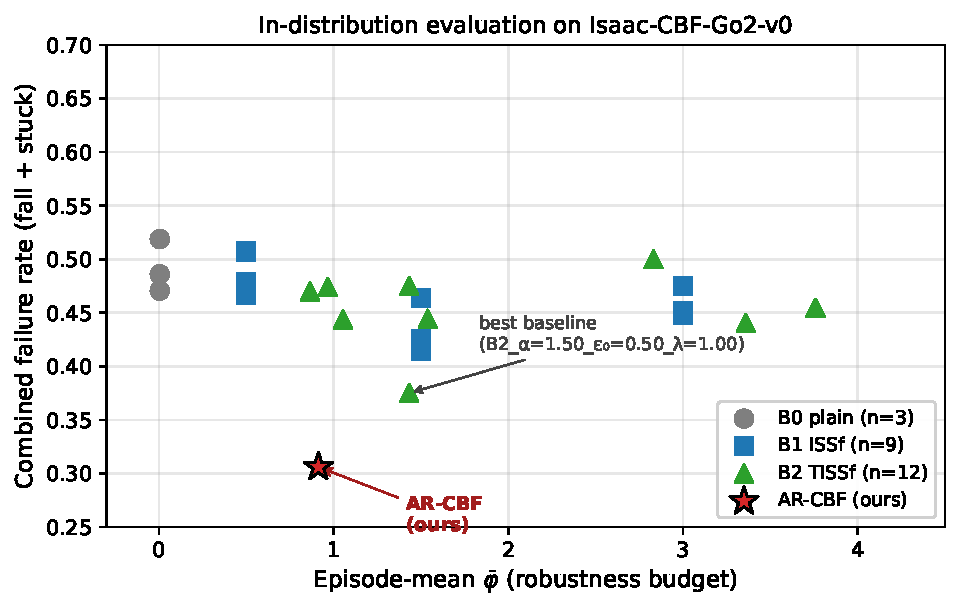
\includegraphics[width=0.7\linewidth]{figures/fig1_baseline_sweep.pdf}
\caption{In-distribution baseline sweep on \texttt{Isaac-CBF-Go2-v0}. Combined
fall+stuck failure rate vs.\ episode-mean $\bar\varphi$ for all $24$ hand-tuned
configurations and \methodname{} (red star). \methodname{} achieves the lowest
combined failure of any of the $25$ configurations evaluated.}
\label{fig:baseline-sweep}
\end{figure}

\subsection{Out-of-Distribution Generalisation}
\label{sec:ood}

We probe generalisation along five single-knob domain shifts, each pushing
exactly one randomisation axis past the training range while keeping every
other axis at its training distribution. The point of single-knob shifts is
diagnostic separation: each shift isolates a specific class of mismatch and
each can be matched to whether the corresponding signal is or is not visible
to the baselines. Plain, ISSf, and TISSf baselines are stateless filters that
read only the current barrier $h(\bx)$ and its gradient; they have no access
to friction, force, mass or scene-velocity history.

\begin{table}[H]
\centering
\small
\begin{tabular}{lcccccc}
\toprule
Eval axis & Type & \methodname{} fall & Stuck & Combined & Best baseline & \textbf{Margin} \\
\midrule
In-dist (ref)     & mixed                  & $0.231$ & $0.075$ & $0.306$ & $0.375$ & $\mathbf{+6.9}$\,pp \\
Slippery          & priv-obs (continuous)  & $0.312$ & $0.099$ & $0.411$ & $0.453$ & $\mathbf{+4.1}$\,pp \\
HighDisturbance   & priv-obs (episodic)    & $0.237$ & $0.104$ & $0.341$ & $0.431$ & $\mathbf{+9.0}$\,pp \\
HeavyCOM          & priv-obs (startup)     & $0.218$ & $0.113$ & $0.331$ & $0.390$ & $\mathbf{+5.9}$\,pp \\
FastObstacles     & priv-obs (grid history)& $0.211$ & $0.128$ & $0.338$ & $0.444$ & $\mathbf{+10.5}$\,pp \\
DensePack         & scene-only             & $0.257$ & $0.081$ & $0.338$ & $0.344$ & $+0.5$\,pp\,(tie) \\
RealisticCompound & all 5 simultaneously   & $0.416$ & $0.084$ & $0.500$ & $0.497$ & $-0.3$\,pp\,(tie) \\
\bottomrule
\end{tabular}
\caption{Single-axis near-OOD generalisation. \methodname{} wins on every
axis whose underlying signal is exposed to it via privileged observation, and
ties on scene-only shifts where baselines have access to the same
$h$-feedback as the teacher.}
\label{tab:ood}
\end{table}

\begin{figure}[H]
\centering
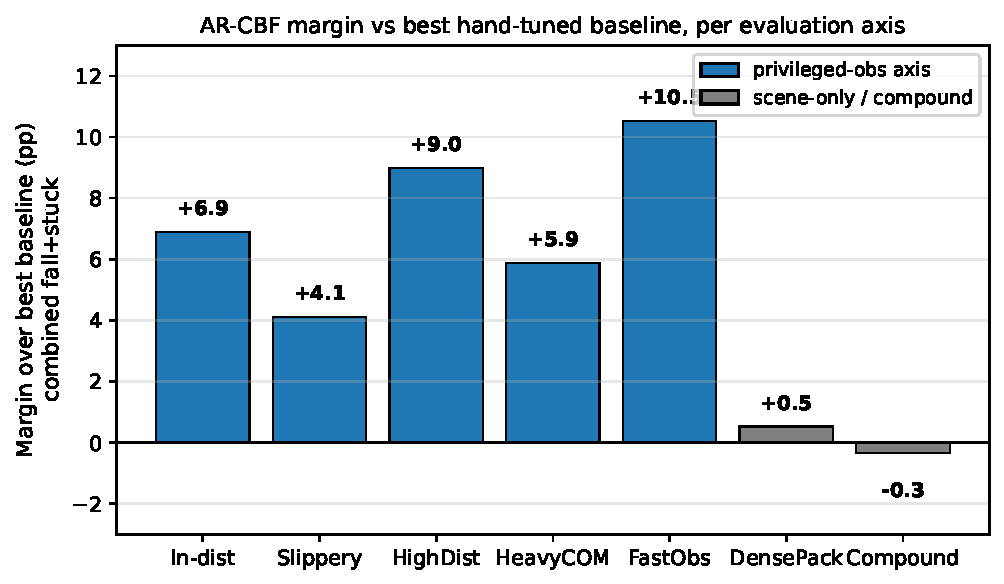
\includegraphics[width=0.78\linewidth]{figures/fig2_ood_margins.pdf}
\caption{Per-axis margin of \methodname{} over the best hand-tuned baseline,
in percentage points of combined fall+stuck failure. Privileged-observation-
aligned axes (blue) show consistent $4$ to $11$\,pp wins. Scene-only axes and
the compound shift (grey) lie within statistical noise of the best baseline.}
\label{fig:ood-margins}
\end{figure}

The pattern in Table~\ref{tab:ood} and Figure~\ref{fig:ood-margins} is sharper
than ``wins everywhere.''
\methodname{} wins by $4$ to $11$ percentage points on every axis whose
disturbance signal is in the privileged-observation vector (friction,
applied force, COM offset, and obstacle motion), and ties the best
baseline within statistical noise on \emph{DensePack}, where the only shift
is scene composition and the baselines see the same $h(\bx)$ that the teacher
does. This is the structural contour of the win: \methodname{} extracts value
specifically from privileged information, exactly as the architecture was
designed to.

% =================================================================
\section{Conclusion and Future Work}
\label{sec:conclusion}

We presented \methodname{}, a method that learns adaptive robustness
parameters for a control barrier function by privileged-observation
reinforcement learning. The learned policy beats the best-tuned hand-coded
baseline by $6.9$ percentage points on combined fall+stuck failure
in-distribution, wins on every privileged observation aligned out of
distribution axis we tested, and ties on scene-only shifts where the playing
field is symmetric. The method is a teacher-side study: distillation to a
proprioceptive student and hardware deployment on the Unitree Go2 are the
obvious next steps, and the infrastructure presented here was deliberately
built with both in mind.

Two limitations follow directly from the design choices above and the
evidence in Section~\ref{sec:results}. First, all evaluations are in
simulation. Sim-to-real transfer of a learned safety filter requires three
things we have not done: (i) calibrating the LiDAR-derived occupancy grid
against real Mid360 data (drop-out and spurious-return rates that we did
not inject during training); (ii) replacing the analytical SDF with a
distance-transformed occupancy grid at deploy time; and (iii) a student
distillation step so that the deployed policy reads only proprioceptive
history rather than privileged dynamics. Each step has a known recipe but
is unevaluated here.

Second, per-axis OOD wins do not compose. Under simultaneous shifts at
modest amplitudes the per-axis margins disappear, indicating that the
encoder was trained on a distribution where each privileged-observation
axis varies independently. The natural fix is to widen training-time
domain randomisation with deliberately correlated joint shifts rather than
independently-sampled marginals. We pursued this direction once and at
fixed compute it produced an under-converged policy that lost on every
axis; the correct fix is wider DR \emph{and} more compute, which we did
not have within the project window. We see this as the most informative
direction for follow-up work, alongside the student-distillation and
hardware-deployment steps already in progress.

% =================================================================
\bibliographystyle{plain}
\bibliography{references}

\end{document}
